\documentclass[12pt,a4paper]{article}
\usepackage[utf8]{inputenc}
\usepackage{amsmath}
\usepackage{amsfonts}
\usepackage{amssymb}

\usepackage{cmap} % для кодировки шрифтов в pdf
\usepackage[T1]{fontenc}
\usepackage{hhline}
\usepackage[unicode]{hyperref}
\usepackage{multirow}
\usepackage{array}
\usepackage{amsmath}
\usepackage{bm}
\usepackage{textcomp}
\usepackage[russian]{babel}
\usepackage{graphicx} % для вставки картинок
\usepackage{amssymb,amsfonts,amsmath,amsthm} % математические дополнения от АМС
\usepackage{indentfirst} % отделять первую строку раздела абзацным отступом тоже
% Поля
\usepackage{geometry}
\geometry{left=2cm}
\geometry{right=1.5cm}
\geometry{top=2.4cm}
\geometry{bottom=2.cm}

%%%%%%%%%%%%%%%%%%%%%%%%%%%%%%%     

\linespread{1.5} % полуторный интервал
\frenchspacing

\begin{document}
	
	\begin{titlepage}
		
		\begin{center}
			\begin{large}
				Санкт-Петербургский Политехнический университет\\ Петра Великого\\
				Институт прикладной математики и механики\\
			\end{large}
			\vspace{0.2cm}
			Высшая школа прикладной математики и вычислительной физики\\
			
		\end{center}
		
		\vspace{3cm}
		\begin{center}
			\textbf{Отчёт\\ по лабораторной работе 4\\ по дисциплине\\ "математическая статистика"}
		\end{center}
		
		\vspace{3cm}
		\vbox{%
			\hfill%
			\vbox{%0
				\hbox{Выполнил студент:}%
				\hbox{\break}
				\hbox{Аникин Алксандр Алексеевич,}%
				\hbox{группа 3630102$\backslash$80201}%
				\hbox{\break}
				\hbox{\break}
				\hbox{Проверил:}
				\hbox{\break}
				\hbox{к.ф.-м.н., доцент}
				\hbox{Баженов Александр Николаевич}
			}%
		} 
		\vfill
		
		\begin{center}
			Санкт-Петербург\\2021
		\end{center}
		
	\end{titlepage}
	\tableofcontents
	\newpage
	
	\listoffigures
	\newpage
	
	\listoftables
	\newpage	
	
	\section{Постановка задачи}
	Для следующих распределений:
	\begin{itemize}
		\item Нормальное распределение $\textit{N}(\textit{x}, 0, 1)$
		\item Распределение Коши $\textit{C}(\textit{x}, 0, 1)$
		\item Распределение Лапласа $\textit{L}(\textit{x}, 0, \frac{1}{\sqrt{2}})$
		\item Распределение Пуассона $\textit{P}(\textit{k}, 10)$
		\item Равномерное распределение $\textit{U}(\textit{x}, -\sqrt{3}, \sqrt{3})$
	\end{itemize}
	Сгенерировать выборки размером 20, 60 и 100 элементов.
	Построить на них эмпирические функции распределения и ядерные
	оценки плотности распределения на отрезке $[-4; 4]$ для непрерывных
	распределений и на отрезке $[6; 14]$ для распределения Пуассона.
	
	\newpage
	
	\section{Теория}
		\subsection{Рассматриваемые распределения}
		Плотности:
		\begin{itemize}
			\item Нормальное распределение:
			\begin{equation}\label{norm}
				\textit{N}(\textit{x}, 0, 1)=\frac{1}{\sqrt{2\pi}}e^{-\frac{x^2}{2}}
			\end{equation}
			
			\item Распределение Коши:
			\begin{equation}\label{cauchy}
				\textit{C}(\textit{x}, 0, 1)=\frac{1}{\pi}\frac{1}{x^2+1}
			\end{equation}
			
			\item Распределение Лапласа:
			\begin{equation}\label{laplace}
				\textit{L}(\textit{x}, 0, \frac{1}{\sqrt{2}})=\frac{1}{\sqrt{2}}e^{-\sqrt{2}|x|}
			\end{equation}
			
			\item Распределение Пуассона:
			\begin{equation}\label{poisson}
				\textit{P}(\textit{k}, 10)=\frac{10^k}{k!}e^{-10}
			\end{equation}
			
			\item Равномерное распределение:
			\begin{equation}\label{uniform}
				\textit{U}(\textit{x}, -\sqrt{3}, \sqrt{3})=
				\left\{
				\begin{array}{l}
					\frac{1}{2\sqrt{3}} \quad \text{при} \quad |x|\leq \sqrt{3}\\
					0 \quad \quad \text{при} \quad |x|>3
				\end{array}
				\right.
			\end{equation}
		\end{itemize}
		
		\subsection{Эмпирическая функция распределения}
			\subsubsection{Статистический ряд}
				Статистическим ряд – последовательность различных элементов выборки
				$z_1, z_2, ... , z_k$, расположенных в возрастающем порядке с указанием частот
				$n_1, n_2, ... , n_k$, с которыми эти элементы содержатся в выборке. Обычно записывается в виде таблицы.
			\subsubsection{Эмпирическая функция распредления}
				Эмпирическая (выборочная) функция распределения  - относительная частота события $X < x$, полученная по данной выборке:
				\begin{equation}
					F^*_n(x)=P^*(X<x)
				\end{equation}
			
			\subsubsection{Нахождение эмпирической функции распределения}
				Для получения относительной частоты $P^*(X<x)$ просуммируем в статистическом ряде, построенном по данной выборке, все частоты
				$n_i$, для которых элементы $z_i$ статистического ряда меньше $x$. Тогда $P^*(X<x)=\frac{1}{n}\sum_{z_i<x}^{ } n_i$. Получаем
				\begin{equation}
					F^*(x)=\frac{1}{n} \sum_{z_i<x}^{ } n_i
				\end{equation}
				$F^*(x)$ - функция распределения дискретной случайной величины $X^*$, заданной таблицей распределения
				\begin{table}[h!]
					\label{distr_table}
					\begin{center}
						\begin{tabular}{|c|c|c|c|c|c|}
							\hline
							X* & $z_1$ & $z_2$ & $z_3$ & $...$ & $z_n$ \\ \hline
							P & $\frac{n_1}{n}$ & $\frac{n_2}{n}$ & $\frac{n_3}{n}$ & $...$ & $\frac{n_k}{n}$ \\ \hline
						\end{tabular}
					\end{center}
					\caption{Таблица распределения}
				\end{table}

				Эмпирическая функция распределения является оценкой, т. е. приближённым значением, генеральной функции распределения
				\begin{equation}
					F^*_n(x) \approx F_X(x)
				\end{equation}
			
		\subsection{Оценки плотности вероятности}
		Оценкой плотности вероятности $f(x)$ называется функция $\hat{f}(x)$, построенная на основе выборки, приближённо равная $f(x)$
		\begin{equation}
			 \hat{f}(x) \approx f(x)
		\end{equation}
		Здесь функция $K(u)$, называемая ядерной (ядром), непрерывна и является плотностью вероятности, $x_1, ... , x_n$ — элементы выборки, $\{n\}$ — любая
		последовательность положительных чисел, обладающая свойствами
		\begin{equation}
			\lim\limits_{n \rightarrow \infty} h_n =0; \quad \lim\limits_{n \rightarrow \infty} \frac{h_n}{n^{-1}} = \infty;
		\end{equation}

		Такие оценки называются непрерывными ядерными \cite{emp1}.
		\break
		Гауссово (нормальное) ядро \cite{emp2}
		\begin{equation}
			K(u)=\frac{1}{\sqrt{2\pi}}e^{\frac{-u^2}{2}}
		\end{equation}
		Правило Сильвермана \cite{emp2}
		\begin{equation}
			h_n1=1.06 \hat{\sigma}n^{-\frac{1}{5}},
		\end{equation}
		где $\hat{\sigma}$ - выборочное стандартное отклонение (корень выборочной дисперсии).
		\newpage
				
	
	\section{Результаты}
		\subsection{Ядерные оценки}
			\begin{figure}[htp]
				{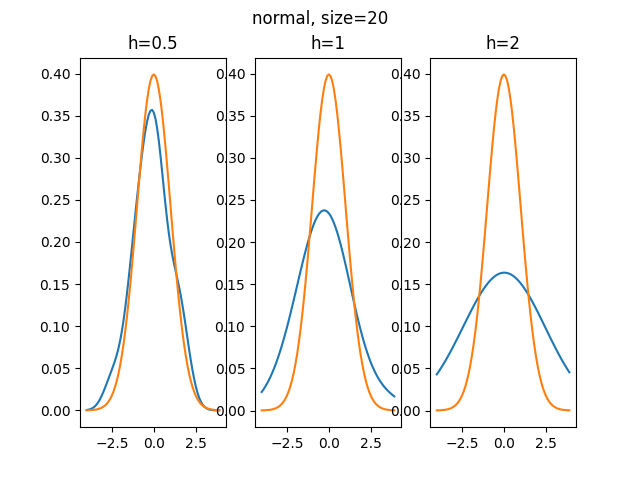
\includegraphics[width=1\linewidth]{../plots/normal_20.png}}
				\caption{Ядерная оценка нормального распределения (\ref{norm}), 20 элементов}
			\end{figure}
			\begin{figure}
				{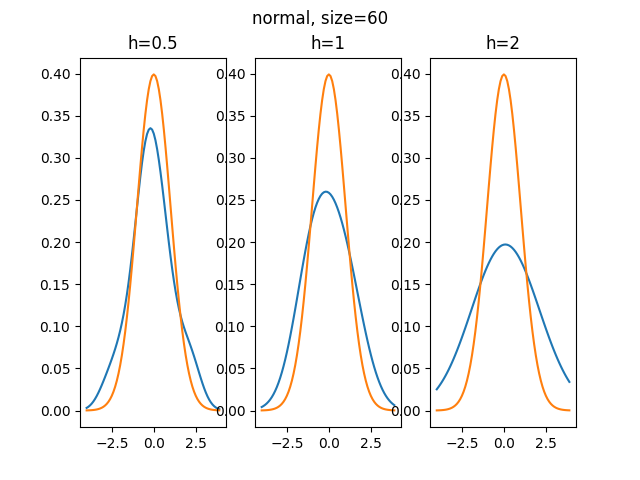
\includegraphics[width=1\linewidth]{../plots/normal_60.png}}
				\caption{Ядерная оценка нормального распределения, 60 элементов}
			\end{figure}
			\newpage
			
			\begin{figure}[htp]
				{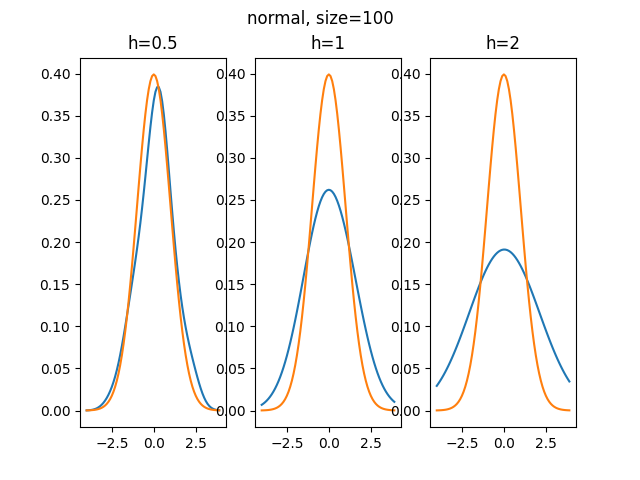
\includegraphics[width=1\linewidth]{../plots/normal_100.png}}
				\caption{Ядерная оценка нормального распределения, 100 элементов}
			\end{figure}
			\begin{figure}
				{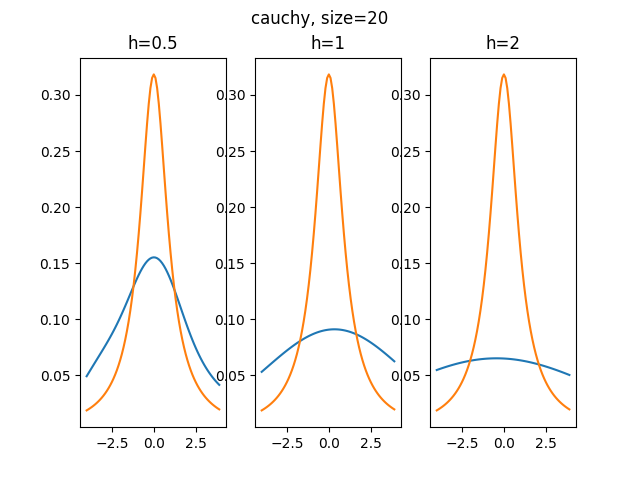
\includegraphics[width=1\linewidth]{../plots/cauchy_20.png}}
				\caption{Ядерная оценка распределения Коши (\ref{cauchy}), 20 элементов}
			\end{figure}
			\newpage
			
			\begin{figure}[htp]
				{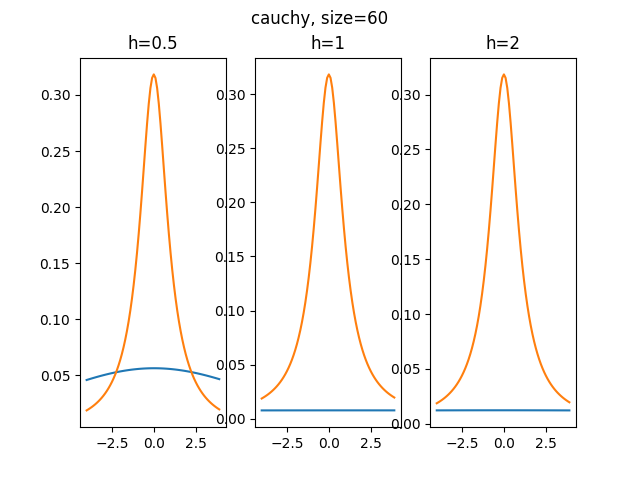
\includegraphics[width=1\linewidth]{../plots/cauchy_60.png}}
				\caption{Ядерная оценка распределения Коши, 60 элементов}
			\end{figure}
			\begin{figure}
				{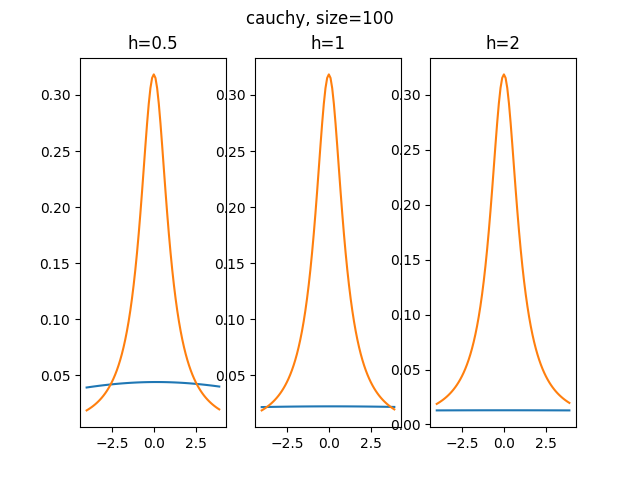
\includegraphics[width=1\linewidth]{../plots/cauchy_100.png}}
				\caption{Ядерная оценка распределения Коши, 100 элементов}
			\end{figure}
			\newpage
			
			\begin{figure}[htp]
				{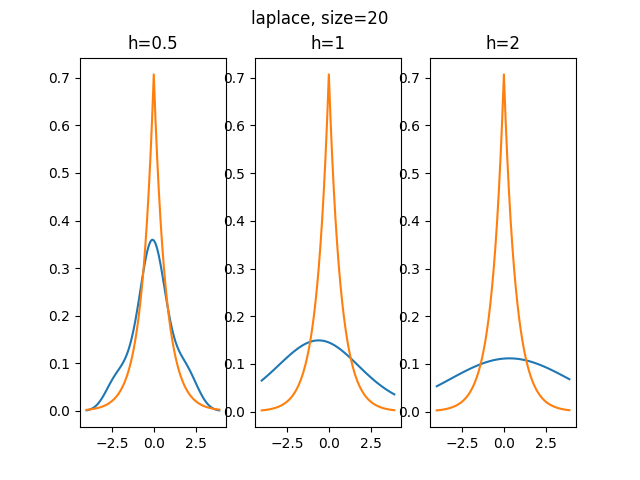
\includegraphics[width=1\linewidth]{../plots/laplace_20.png}}
				\caption{Ядерная оценка распределения Лапласа (\ref{laplace}), 20 элементов}
			\end{figure}
			\begin{figure}
				{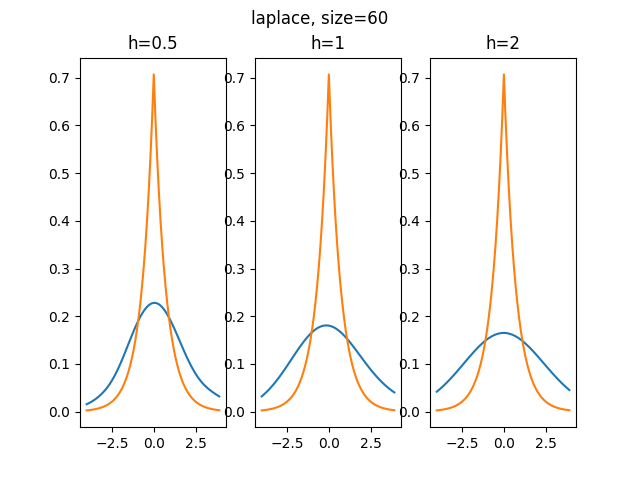
\includegraphics[width=1\linewidth]{../plots/laplace_60.png}}
				\caption{Ядерная оценка распределения Лапласа, 60 элементов}
			\end{figure}
		
			\begin{figure}[htp]
				{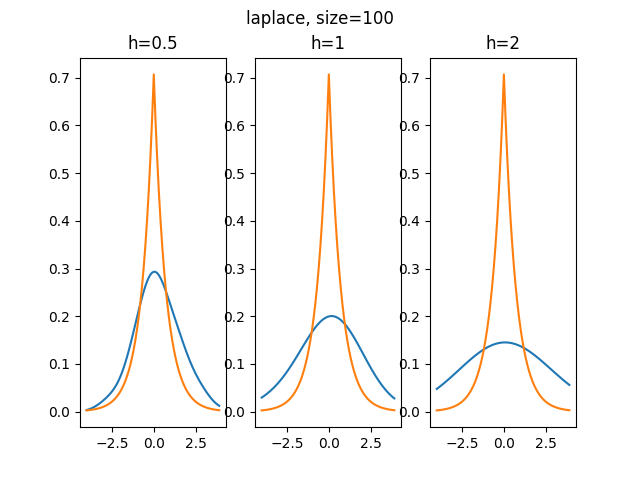
\includegraphics[width=1\linewidth]{../plots/laplace_100.png}}
				\caption{Ядерная оценка распределения Лапласа, 100 элементов}
			\end{figure}
			\begin{figure}
				{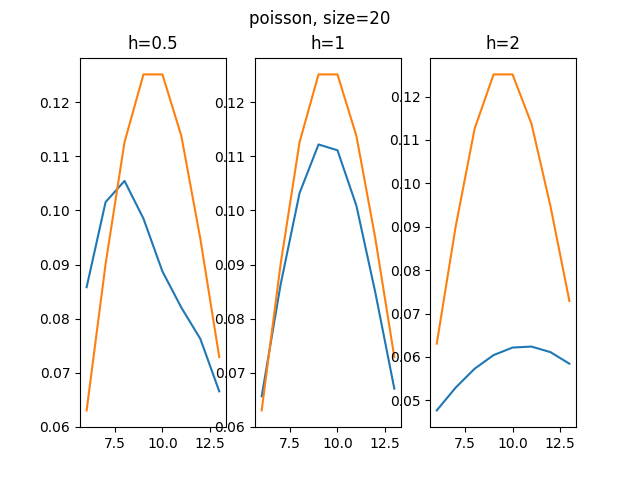
\includegraphics[width=1\linewidth]{../plots/poisson_20.png}}
				\caption{Ядерная оценка распределения Пуассона (\ref{poisson}), 20 элементов}
			\end{figure}
		
			\begin{figure}[htp]
				{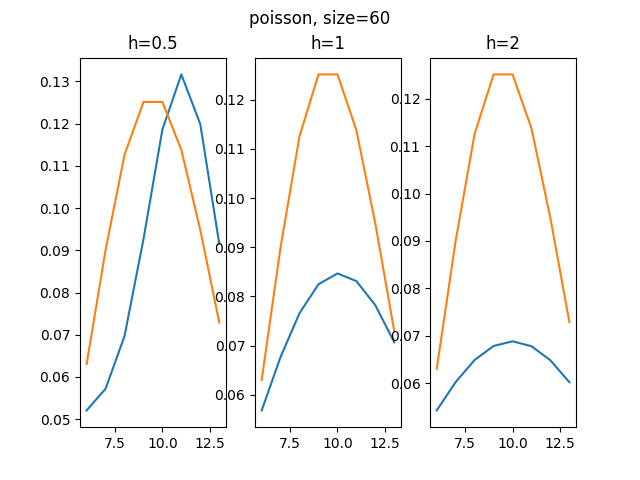
\includegraphics[width=1\linewidth]{../plots/poisson_60.png}}
				\caption{Ядерная оценка распределения Лапласа, 60 элементов}
			\end{figure}
			\begin{figure}
				{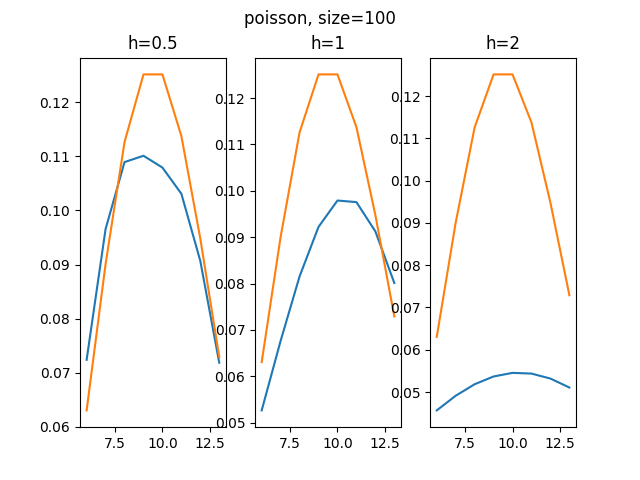
\includegraphics[width=1\linewidth]{../plots/poisson_100.png}}
				\caption{Ядерная оценка распределения Пуассона, 100 элементов}
			\end{figure}
			
			\begin{figure}[htp]
				{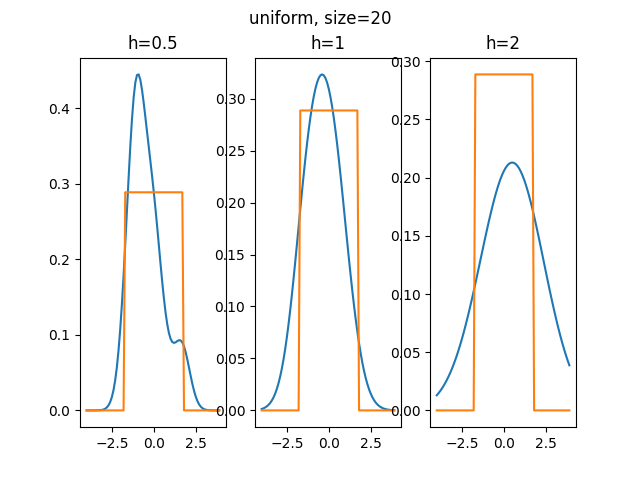
\includegraphics[width=1\linewidth]{../plots/uniform_20.png}}
				\caption{Ядерная оценка равномерного распределения (\ref{uniform}), 20 элементов}
			\end{figure}
			\begin{figure}
				{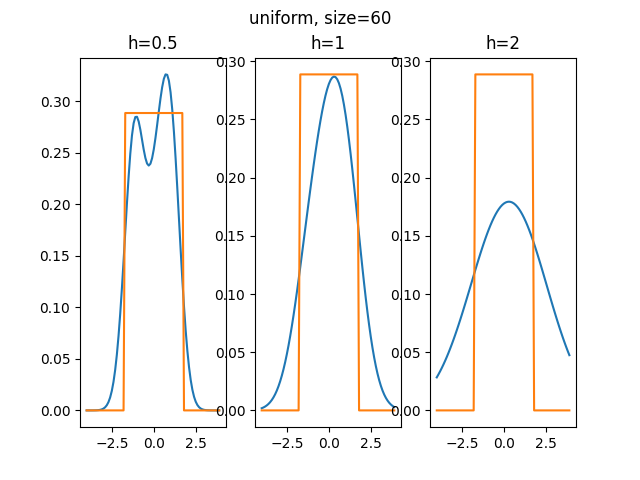
\includegraphics[width=1\linewidth]{../plots/uniform_60.png}}
				\caption{Ядерная оценка равномерного распределения, 60 элементов}
			\end{figure}
			\clearpage
			\newpage
			
			\begin{figure}[htp]
				{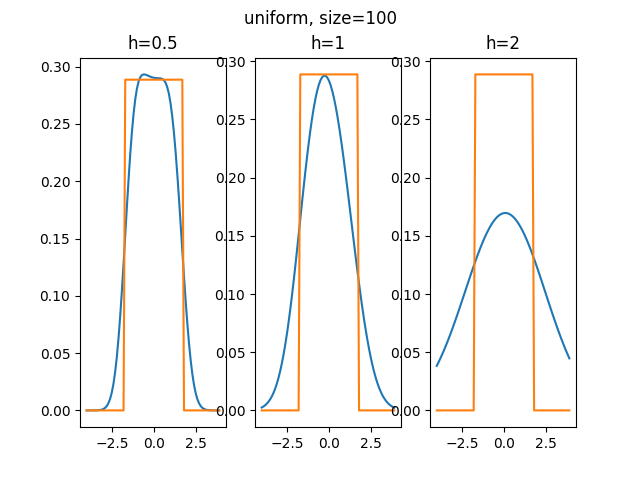
\includegraphics[width=1\linewidth]{../plots/uniform_100.png}}
				\caption{Ядерная оценка равномерного распределения, 100 элементов}
			\end{figure}
			
			\newpage
			\subsection{Эмпирические функции распределения}
			
			\centering{
				\begin{figure}[htp]
					\begin{minipage}[h]{0.3\linewidth}
						\centering{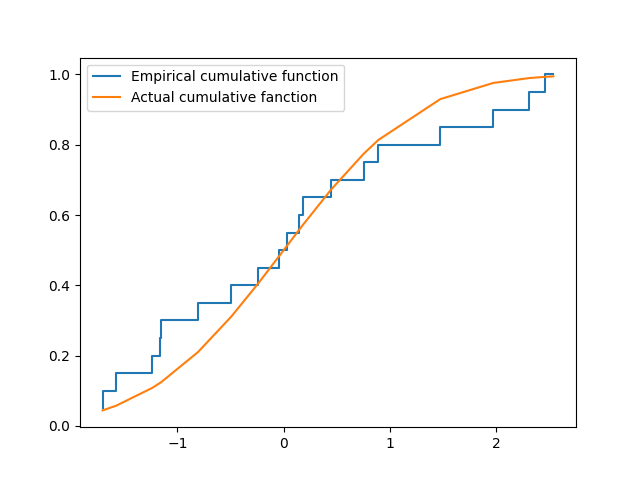
\includegraphics[width=1.25\linewidth]{../plots/normal_cum_20.png}}\\
					\end{minipage}
					\hfill
					\begin{minipage}[h]{0.3\linewidth}
						\centering{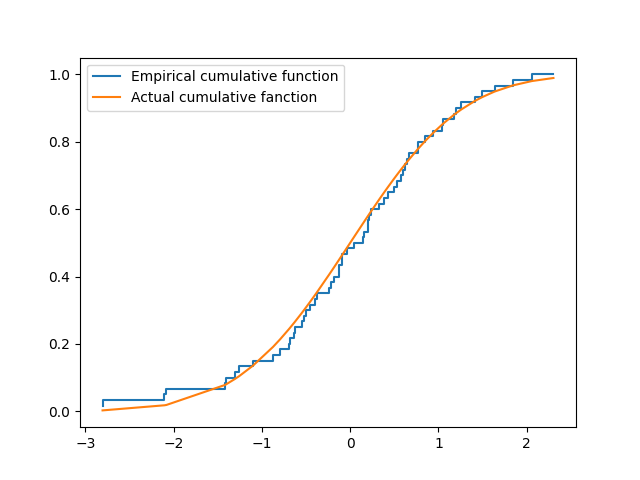
\includegraphics[width=1.25\linewidth]{../plots/normal_cum_60.png}}\\
					\end{minipage}
					\hfill
					\begin{minipage}[h]{0.3\linewidth}
						\centering{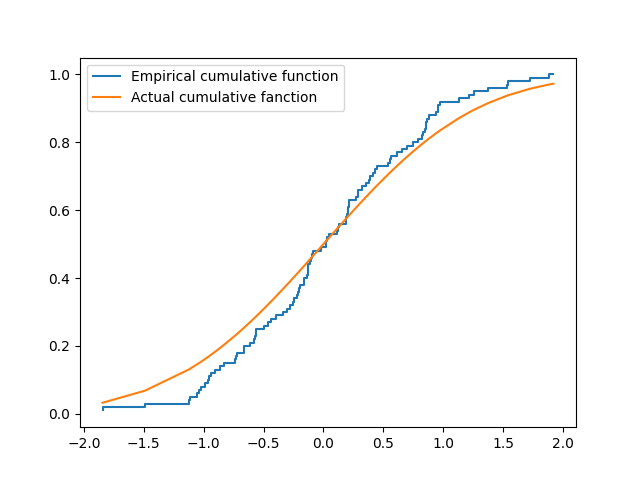
\includegraphics[width=1.25\linewidth]{../plots/normal_cum_100.png}}\\
					\end{minipage}
					\caption{Нормальное распределение (\ref{norm}), графики фактической и эмпирической функций распределения}
					\label{ris:normal_cum}
				\end{figure}
			}
		
			\centering{
				\begin{figure}[htp]
					\begin{minipage}[h]{0.3\linewidth}
						\centering{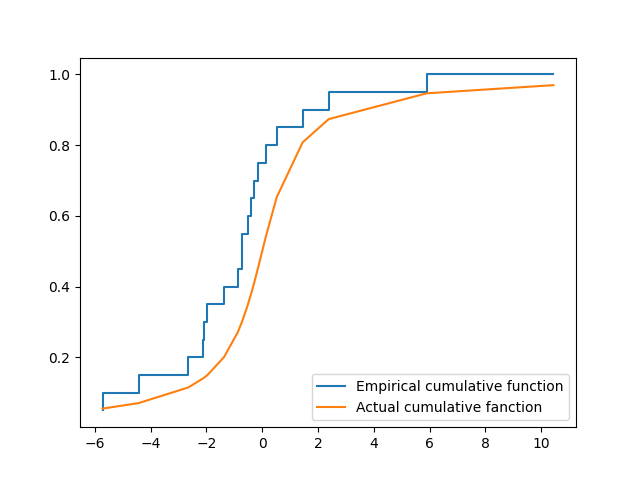
\includegraphics[width=1.25\linewidth]{../plots/cauchy_cum_20.png}}\\
					\end{minipage}
					\hfill
					\begin{minipage}[h]{0.3\linewidth}
						\centering{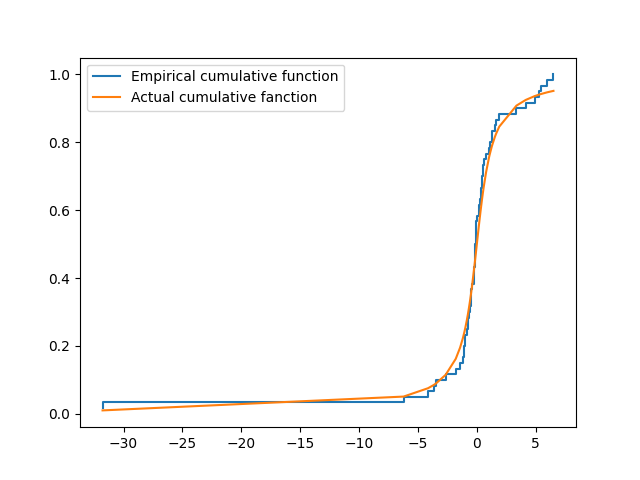
\includegraphics[width=1.25\linewidth]{../plots/cauchy_cum_60.png}}\\
					\end{minipage}
					\hfill
					\begin{minipage}[h]{0.3\linewidth}
						\centering{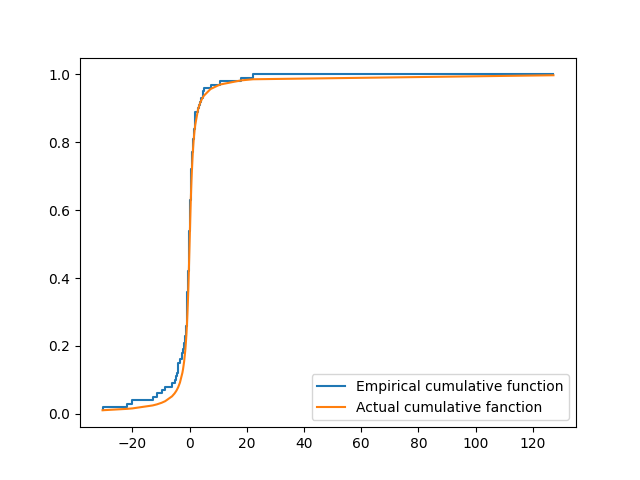
\includegraphics[width=1.25\linewidth]{../plots/cauchy_cum_100.png}}\\
					\end{minipage}
					\caption{Распределение Коши (\ref{cauchy}), графики фактической и эмпирической функций распределения}
					\label{ris:cauchy_cum}
				\end{figure}
			}
		
			\centering{
				\begin{figure}[htp]
					\begin{minipage}[h]{0.3\linewidth}
						\centering{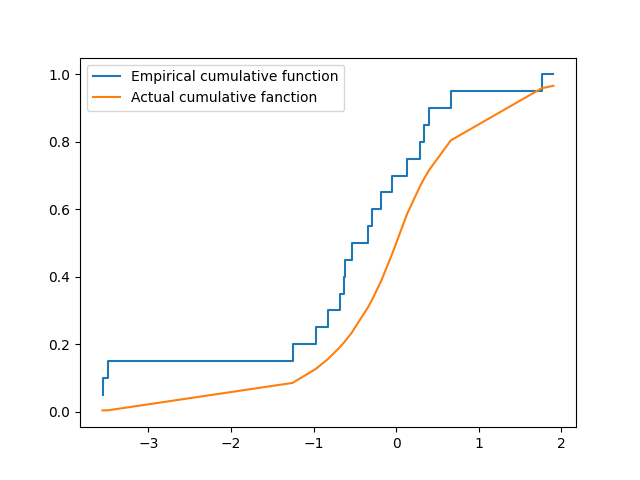
\includegraphics[width=1.25\linewidth]{../plots/laplace_cum_20.png}}\\
					\end{minipage}
					\hfill
					\begin{minipage}[h]{0.3\linewidth}
						\centering{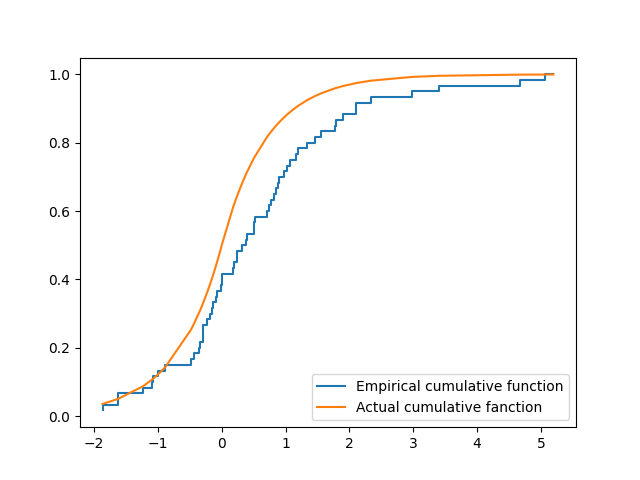
\includegraphics[width=1.25\linewidth]{../plots/laplace_cum_60.png}}\\
					\end{minipage}
					\hfill
					\begin{minipage}[h]{0.3\linewidth}
						\centering{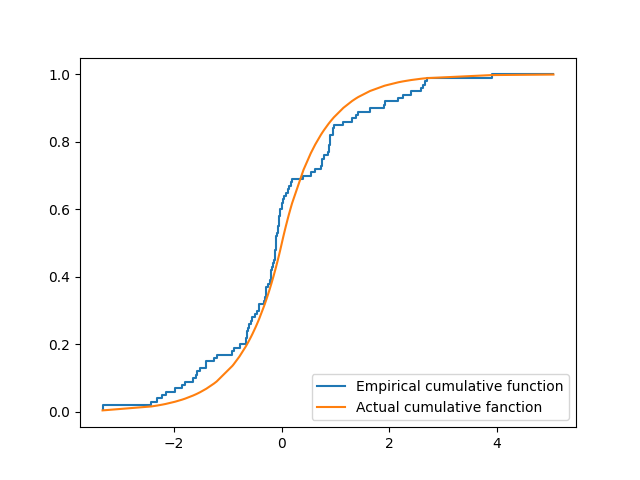
\includegraphics[width=1.25\linewidth]{../plots/laplace_cum_100.png}}\\
					\end{minipage}
					\caption{Распределение Лапласа (\ref{laplace}), графики фактической и эмпирической функций распределения}
					\label{ris:laplace_cum}
				\end{figure}
			}
		
			\centering{
				\begin{figure}[htp]
					\begin{minipage}[h]{0.3\linewidth}
						\centering{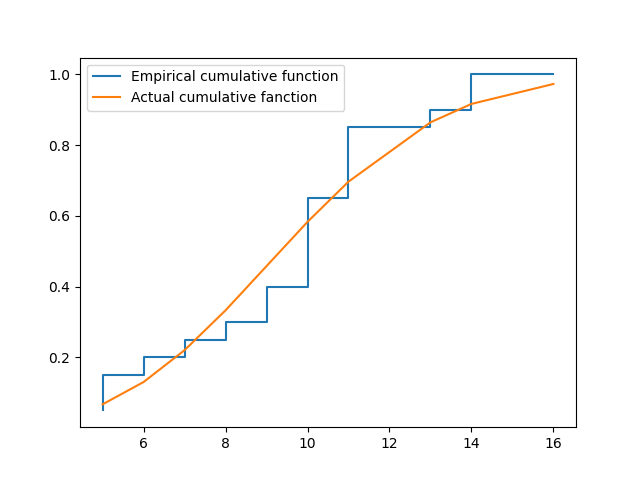
\includegraphics[width=1.25\linewidth]{../plots/poisson_cum_20.png}}\\
					\end{minipage}
					\hfill
					\begin{minipage}[h]{0.3\linewidth}
						\centering{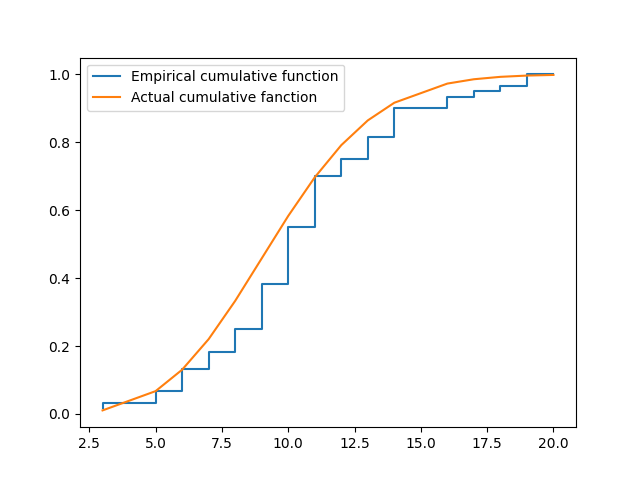
\includegraphics[width=1.25\linewidth]{../plots/poisson_cum_60.png}}\\
					\end{minipage}
					\hfill
					\begin{minipage}[h]{0.3\linewidth}
						\centering{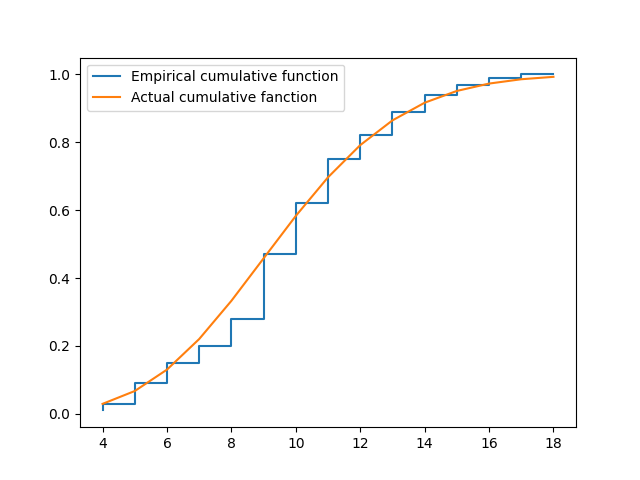
\includegraphics[width=1.25\linewidth]{../plots/poisson_cum_100.png}}\\
					\end{minipage}
					\caption{Распределение Пуассона (\ref{poisson}), графики фактической и эмпирической функций распределения}
					\label{ris:poisson_cum}
				\end{figure}
			}
			
			\centering{
				\begin{figure}[htptp]
					\begin{minipage}[h]{0.3\linewidth}
						\centering{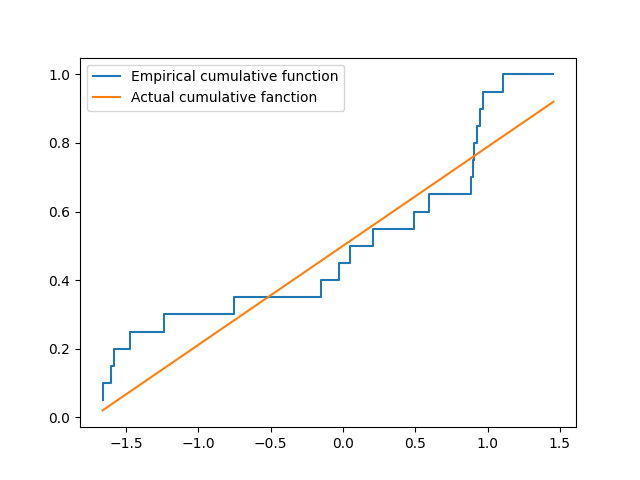
\includegraphics[width=1.25\linewidth]{../plots/uniform_cum_20.png}}\\
					\end{minipage}
					\hfill
					\begin{minipage}[h]{0.3\linewidth}
						\centering{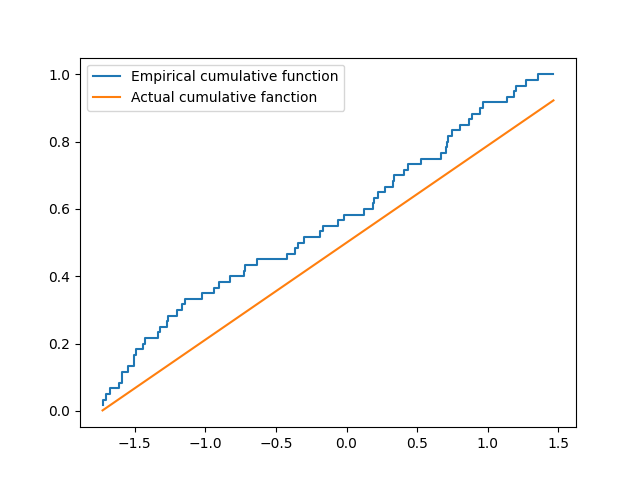
\includegraphics[width=1.25\linewidth]{../plots/uniform_cum_60.png}}\\
					\end{minipage}
					\hfill
					\begin{minipage}[h]{0.3\linewidth}
						\centering{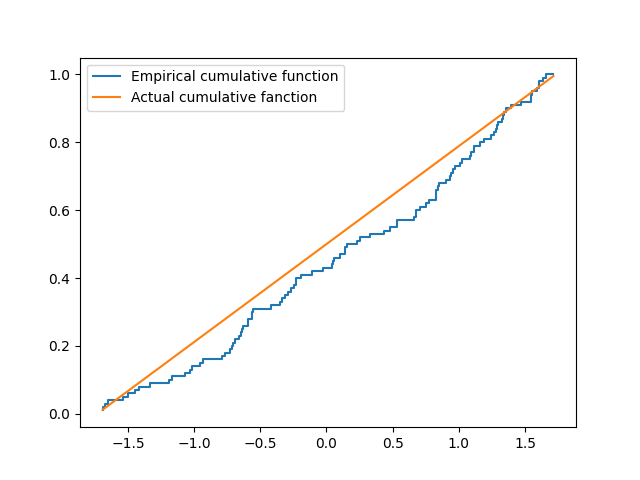
\includegraphics[width=1.25\linewidth]{../plots/uniform_cum_100.png}}\\
					\end{minipage}
					\caption{Равномерное распредление (\ref{uniform}), графики фактической и эмпирической функций распределения}
					\label{ris:uniform_cum}
				\end{figure}
			}
			\clearpage
			\newpage
	
	\begin{thebibliography}{1}
		\addcontentsline{toc}{section}{\bibname}
		\bibitem{emp1}  Вероятностные разделы математики. Учебник для бакалавров технических направлений.//Под ред. Максимова Ю.Д. — Спб.: «Иван Федоров»,
		2001. — 592 c., илл.
		\bibitem{emp2} Анатольев, Станислав (2009) «Непараметрическая регрессия», Квантиль, №7, стр. 37-52.
	\end{thebibliography}
\end{document}